\documentclass[UTF8,a4paper,10pt]{article}

\usepackage{ctex}
\usepackage{physics}
\usepackage{graphicx}
\usepackage[subfigure,AllowH]{graphfig} %图片相关

\title{基于Latex写作的大炮打蚊子研究}
\author{waacing}

\begin{document}
	\maketitle 
	我也不知道写啥随便写写。
	\section{公式}
	\subsection{公式对齐}
	运算过程/公式太长的运算符号对齐:
	\begin{equation} \label{}
		\begin{aligned}
			\frac{dG}{dt}&=\sum(\dot{\overline{r_i}}\cdot \overline{p_i} + \dot{\overline{p_i}} \cdot \overline{r_i} ) \\
			&=\sum(\overline{F_i}\cdot \overline{r_i} + \overline{p_i} \cdot \overline{v_i}) \\
			&=\sum(\overline{F_i}\cdot \overline{r_i} + mv_i^2)
		\end{aligned}
	\end{equation}
	
	\subsection{大括号}
	\begin{equation}
		sample = \left\{ 
		\begin{aligned}
			r(t+\Delta t)&=r(t)+v(t)\Delta t+\frac{1}{2}a(t)\Delta t^2 \\
			v(t+\Delta t)&=v(t)+\frac{1}{2}[a(t)+a(t+\Delta t)]\Delta t
		\end{aligned}
		\right.
	\end{equation}
	
	\subsection{矩阵}
	\begin{equation} 
		\begin{gathered}
			\vb{v} \times \vb{u} = 
			\begin{aligned}
				\begin{vmatrix} 
					i & j & k \\ 
					v_x & v_y  & v_z \\ 
					u_x & u_y & u_z
				\end{vmatrix}
			\end{aligned}
		\end{gathered}
	\end{equation}

	\section{KAI模型}
\begin{enumerate}
	\item $\Delta P(t) = 2P_s[1-exp{(-t/t_0)^n}]$
	\item 有缺陷时,畴不能无限扩展,不能使用KAI模型
\end{enumerate} 
	
	\section{图片}
	\subsection{插入不同路径的图片}
	\begin{figure} [!h] % [!h]控制图片随着代码的位置改变
		\centering % 图片居中
		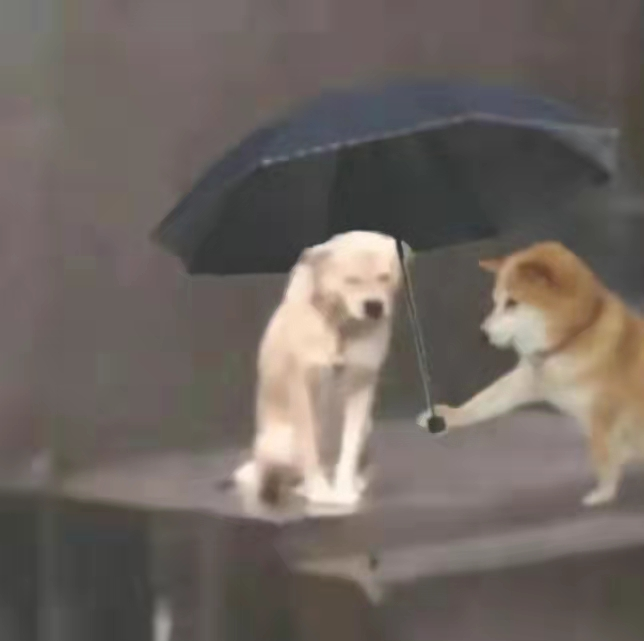
\includegraphics[width=0.7\linewidth]{fig/1} % 0.7\linewidth表示行距的0.7倍,fig/force表示读取存在fig文件夹中名为force的图片
		\caption{随便写写} %用来引用图片
	\end{figure}

	\subsection{插入子图}
	\begin{figure}[hb]
		\centering
		\subfigure[能量随温度变化关系图]{  % 子图的批注
			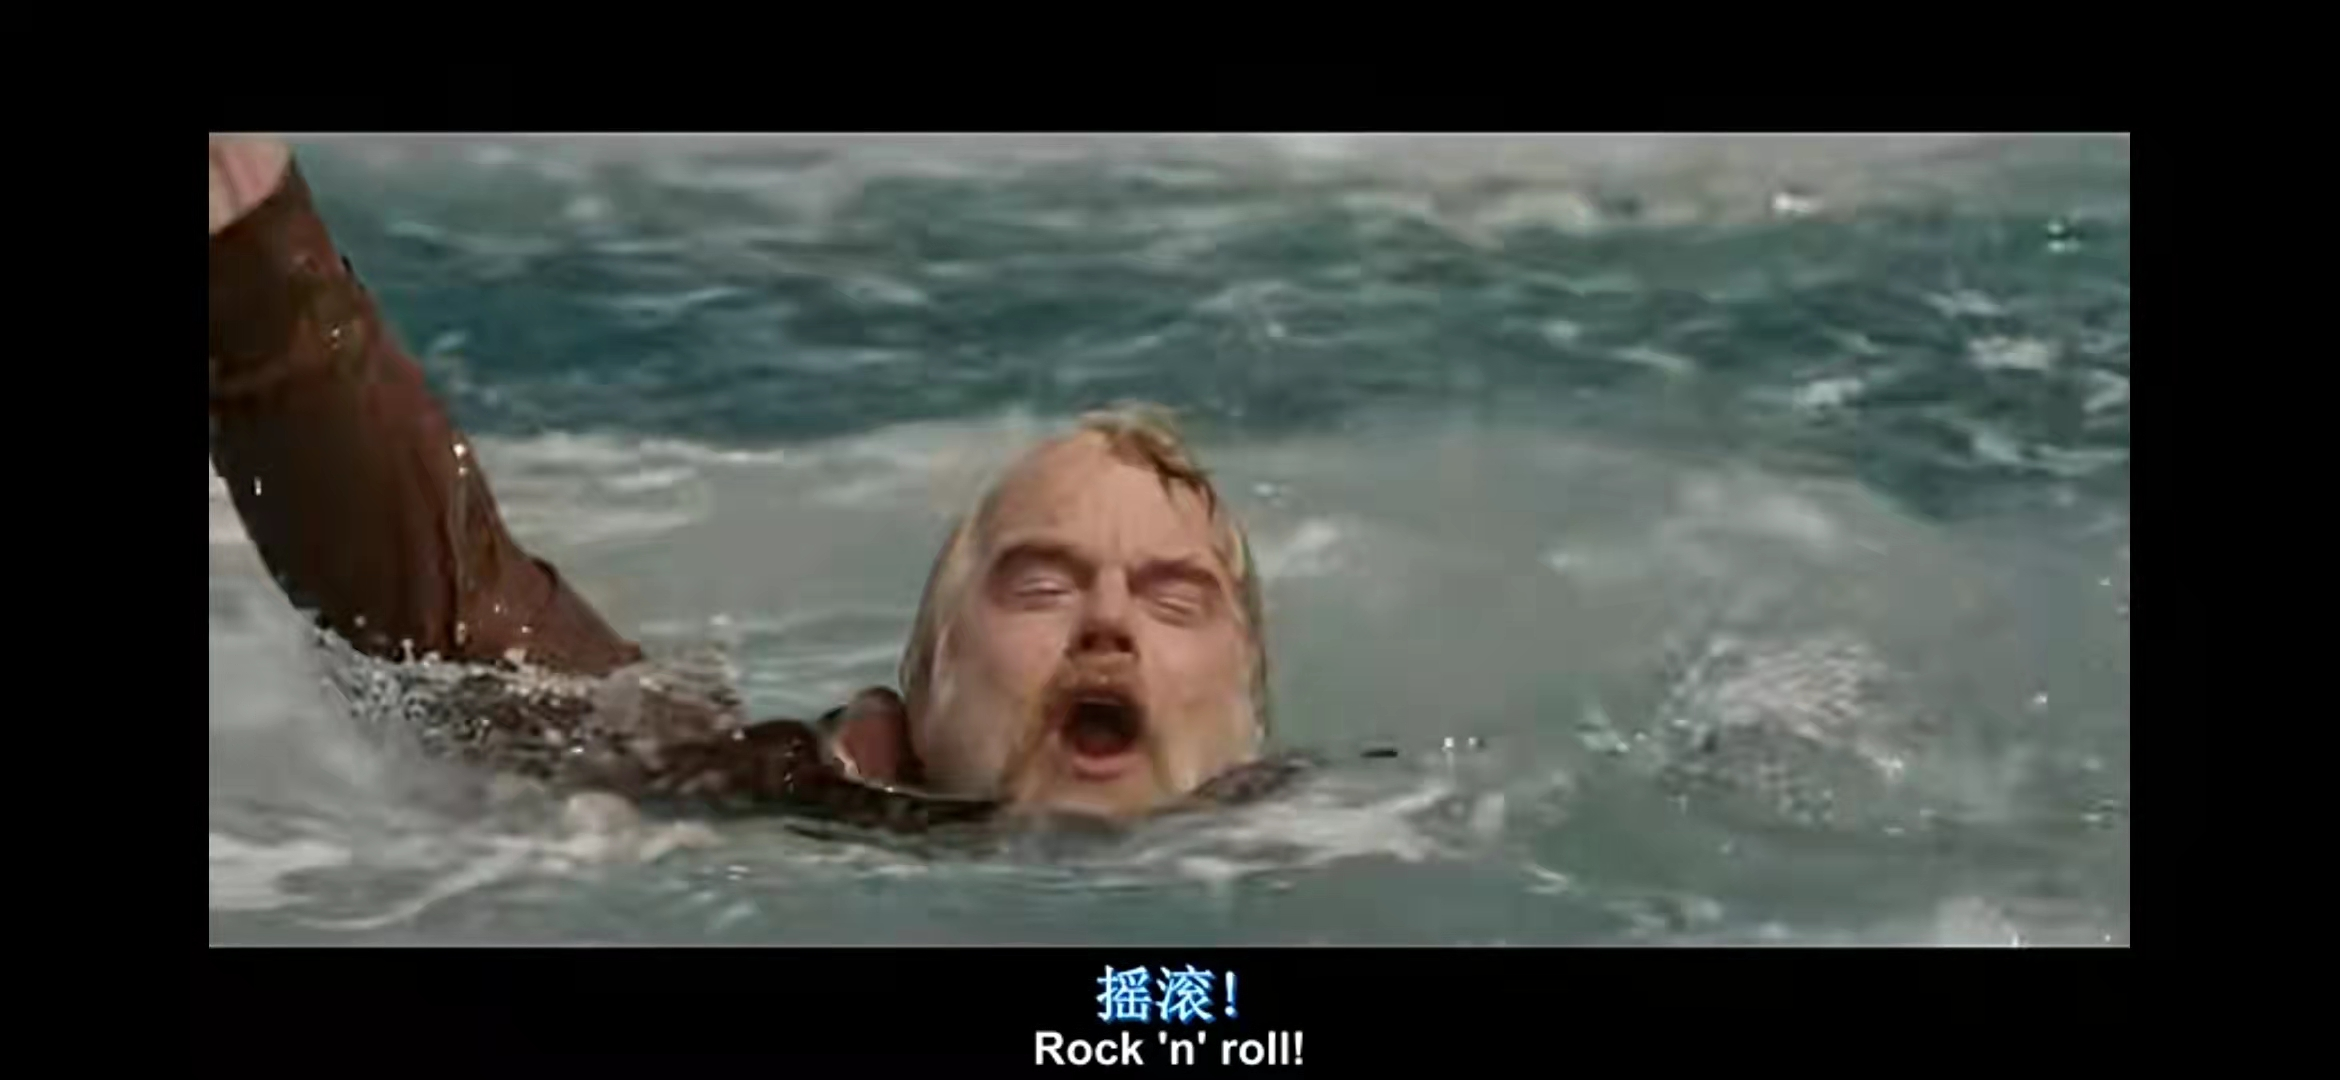
\includegraphics[scale=0.05]{fig/2} \label{1} %图形的缩放因子,设定 scale=0.2 会使插入的图形的大小为其自然大小的0.2倍。
		}
		\quad
		\subfigure[磁化强度与温度的关系图]{
			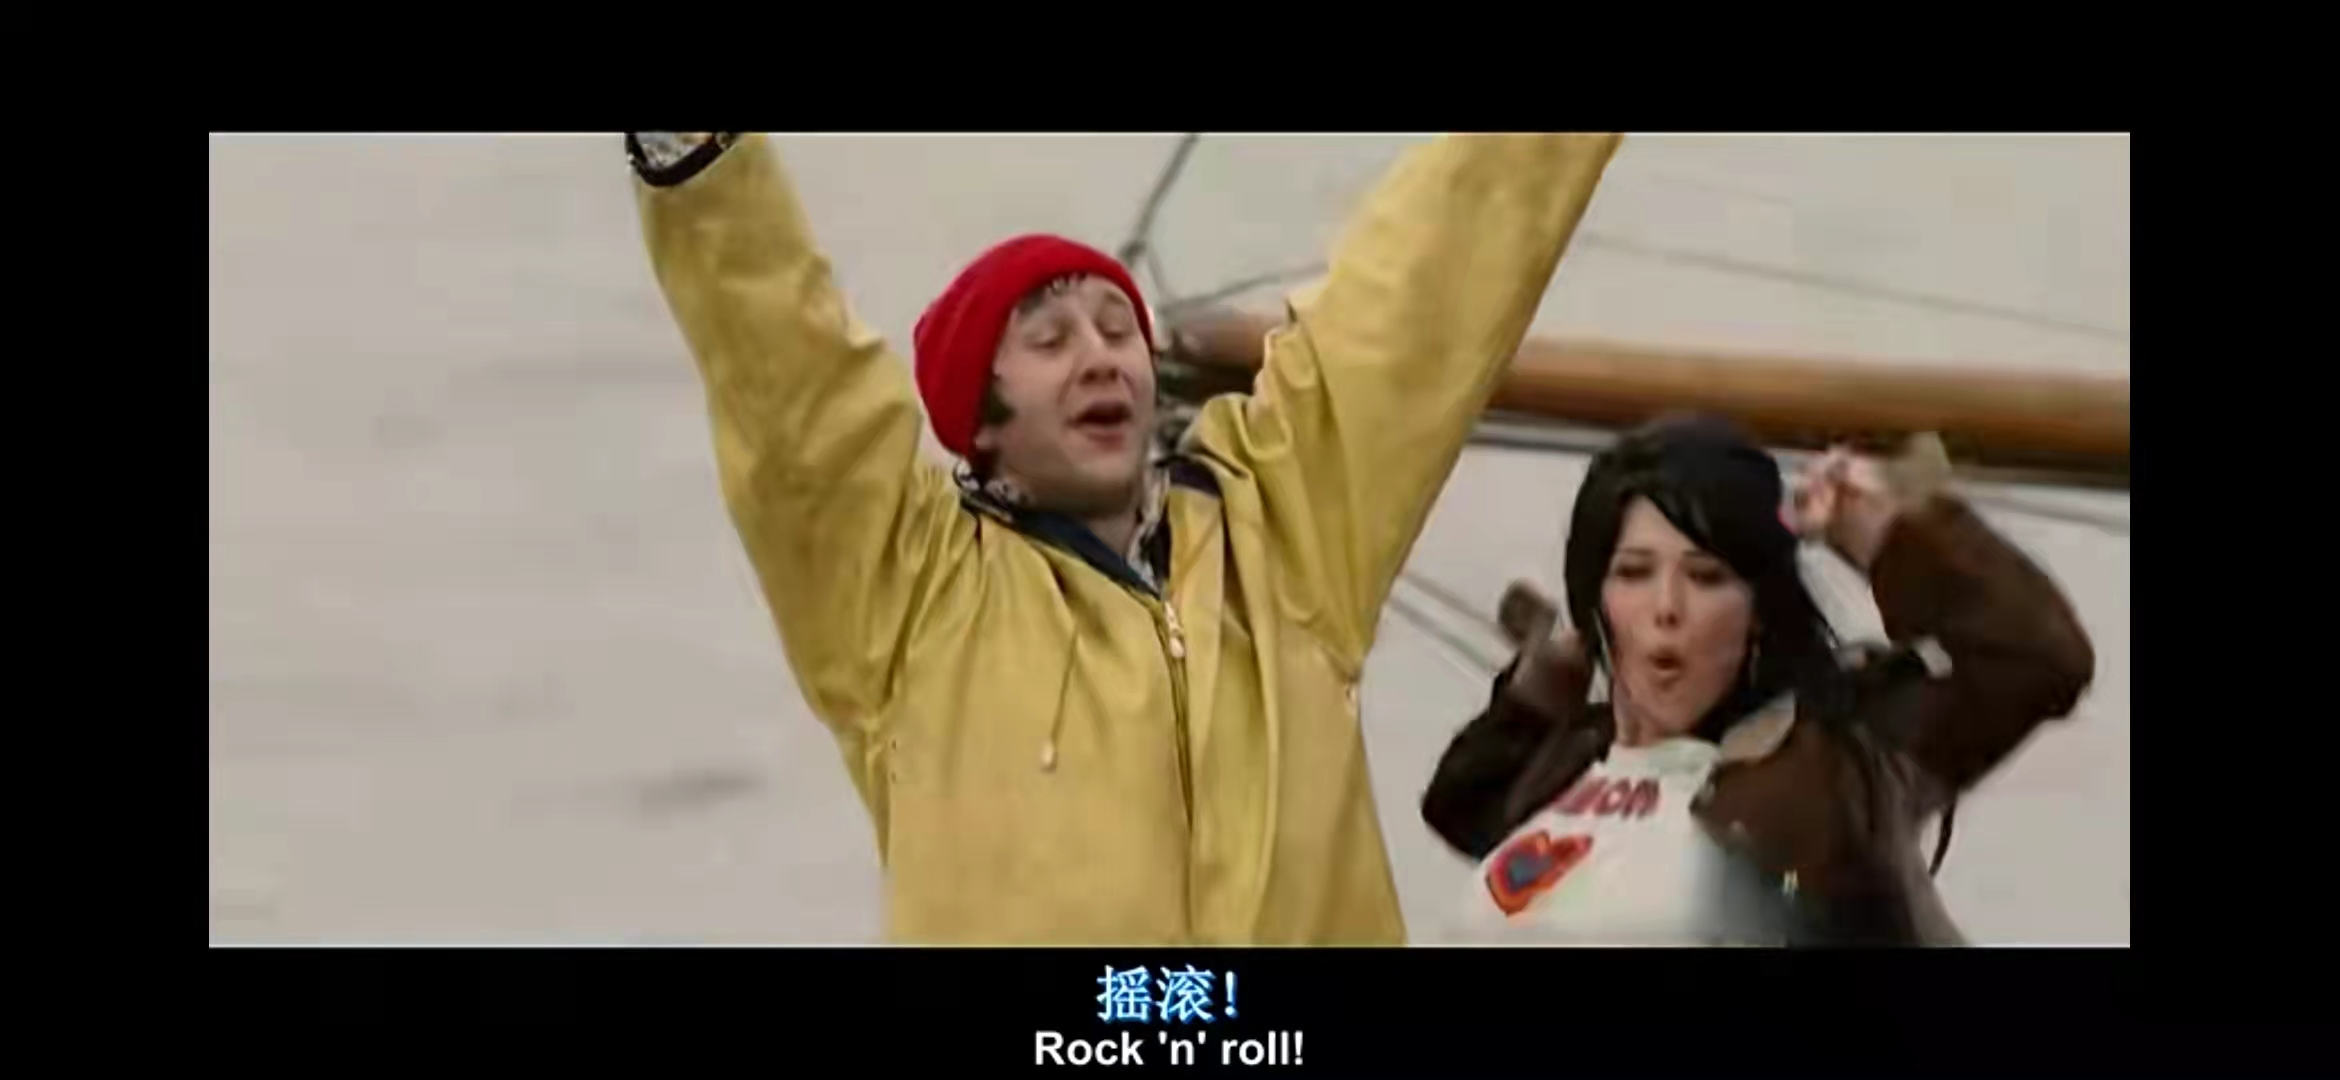
\includegraphics[scale=0.05]{fig/3} \label{2}
		}
		\quad
		\subfigure[热容与温度的关系图]{
			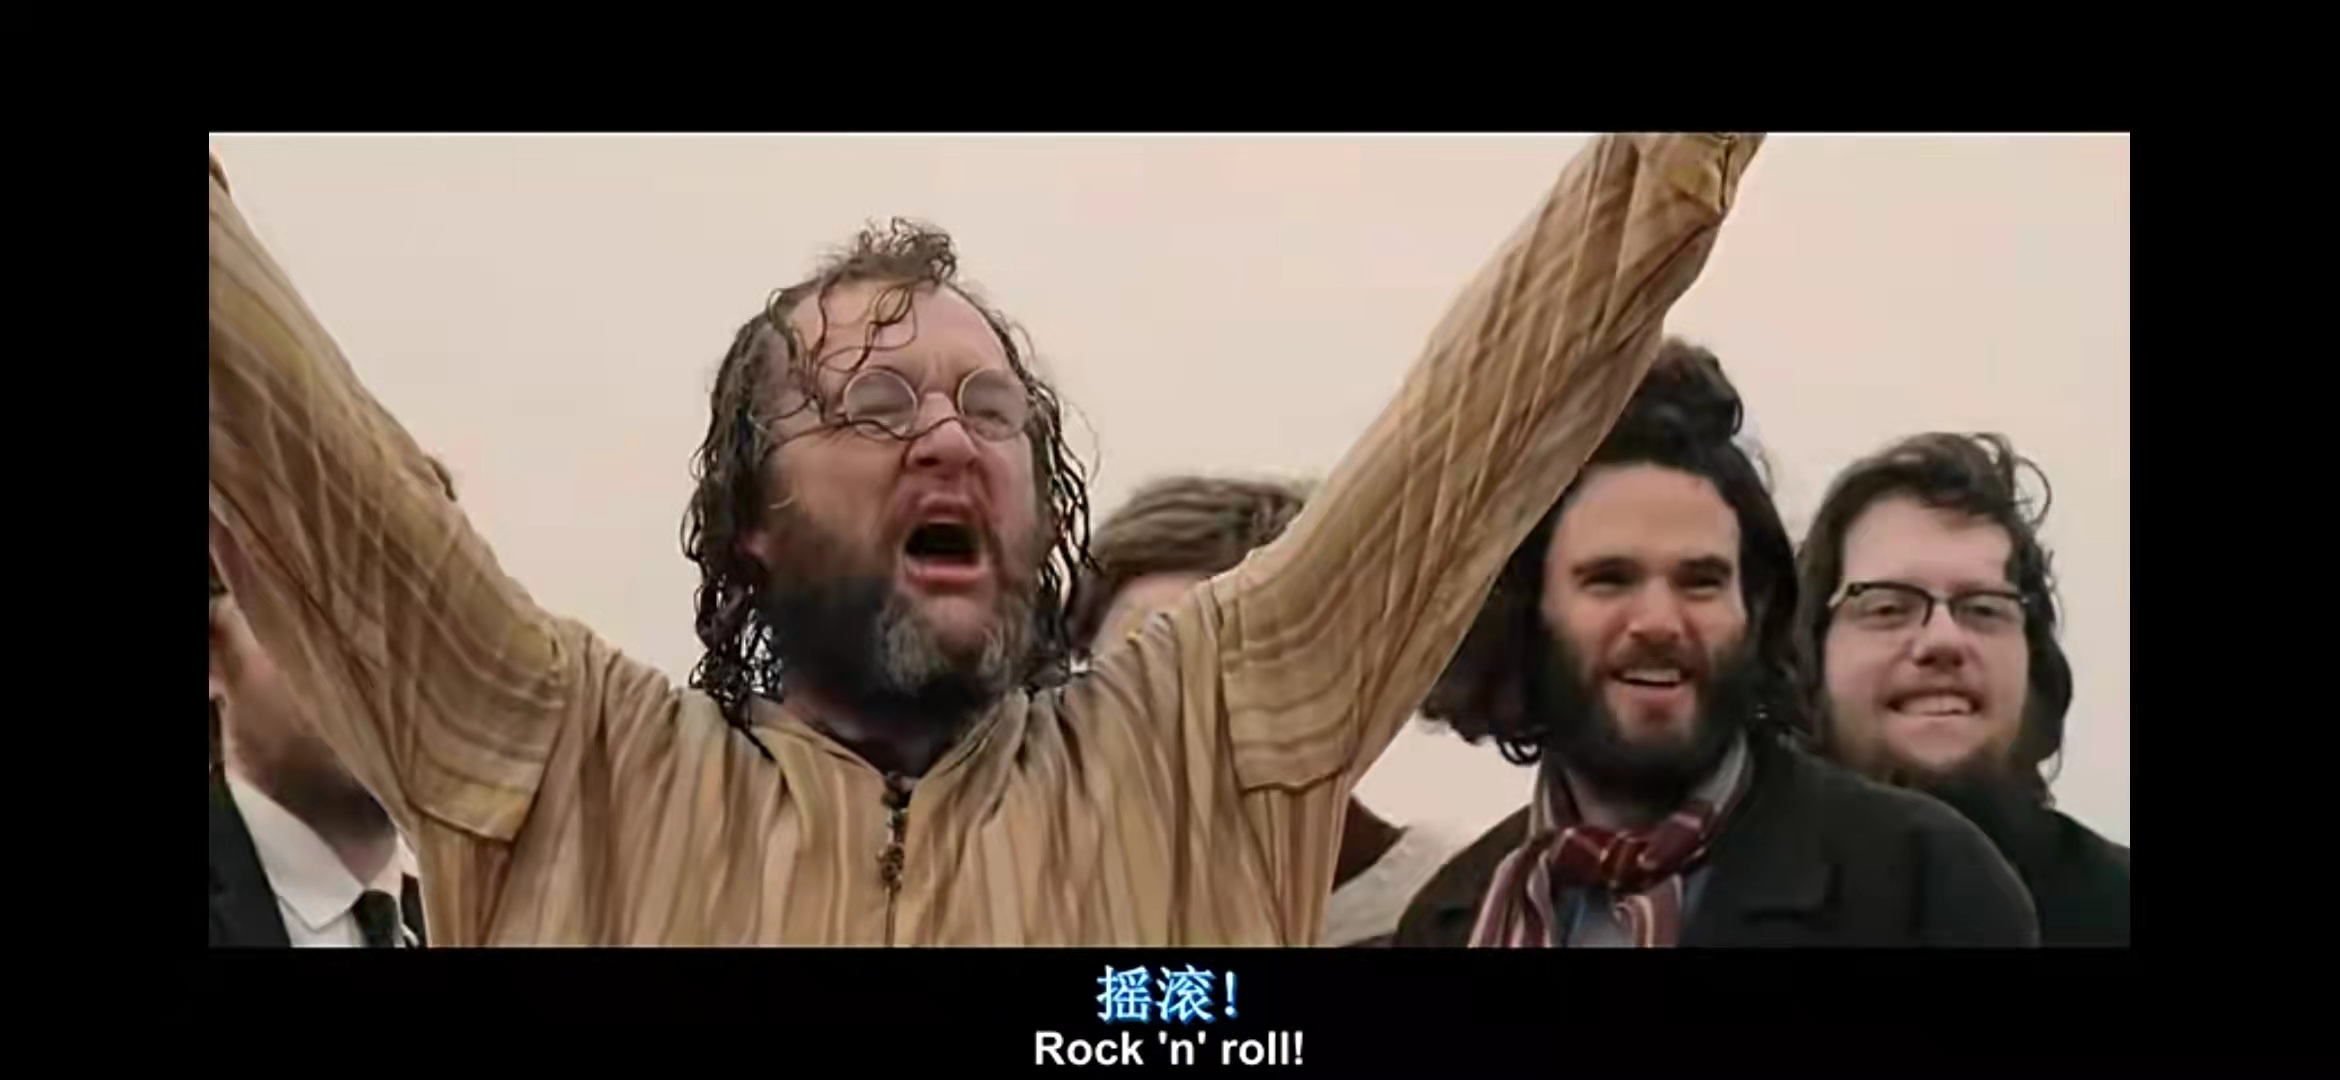
\includegraphics[scale=0.05]{fig/4}\label{3}
		}
		\quad
		\subfigure[磁化率与温度的关系图]{
			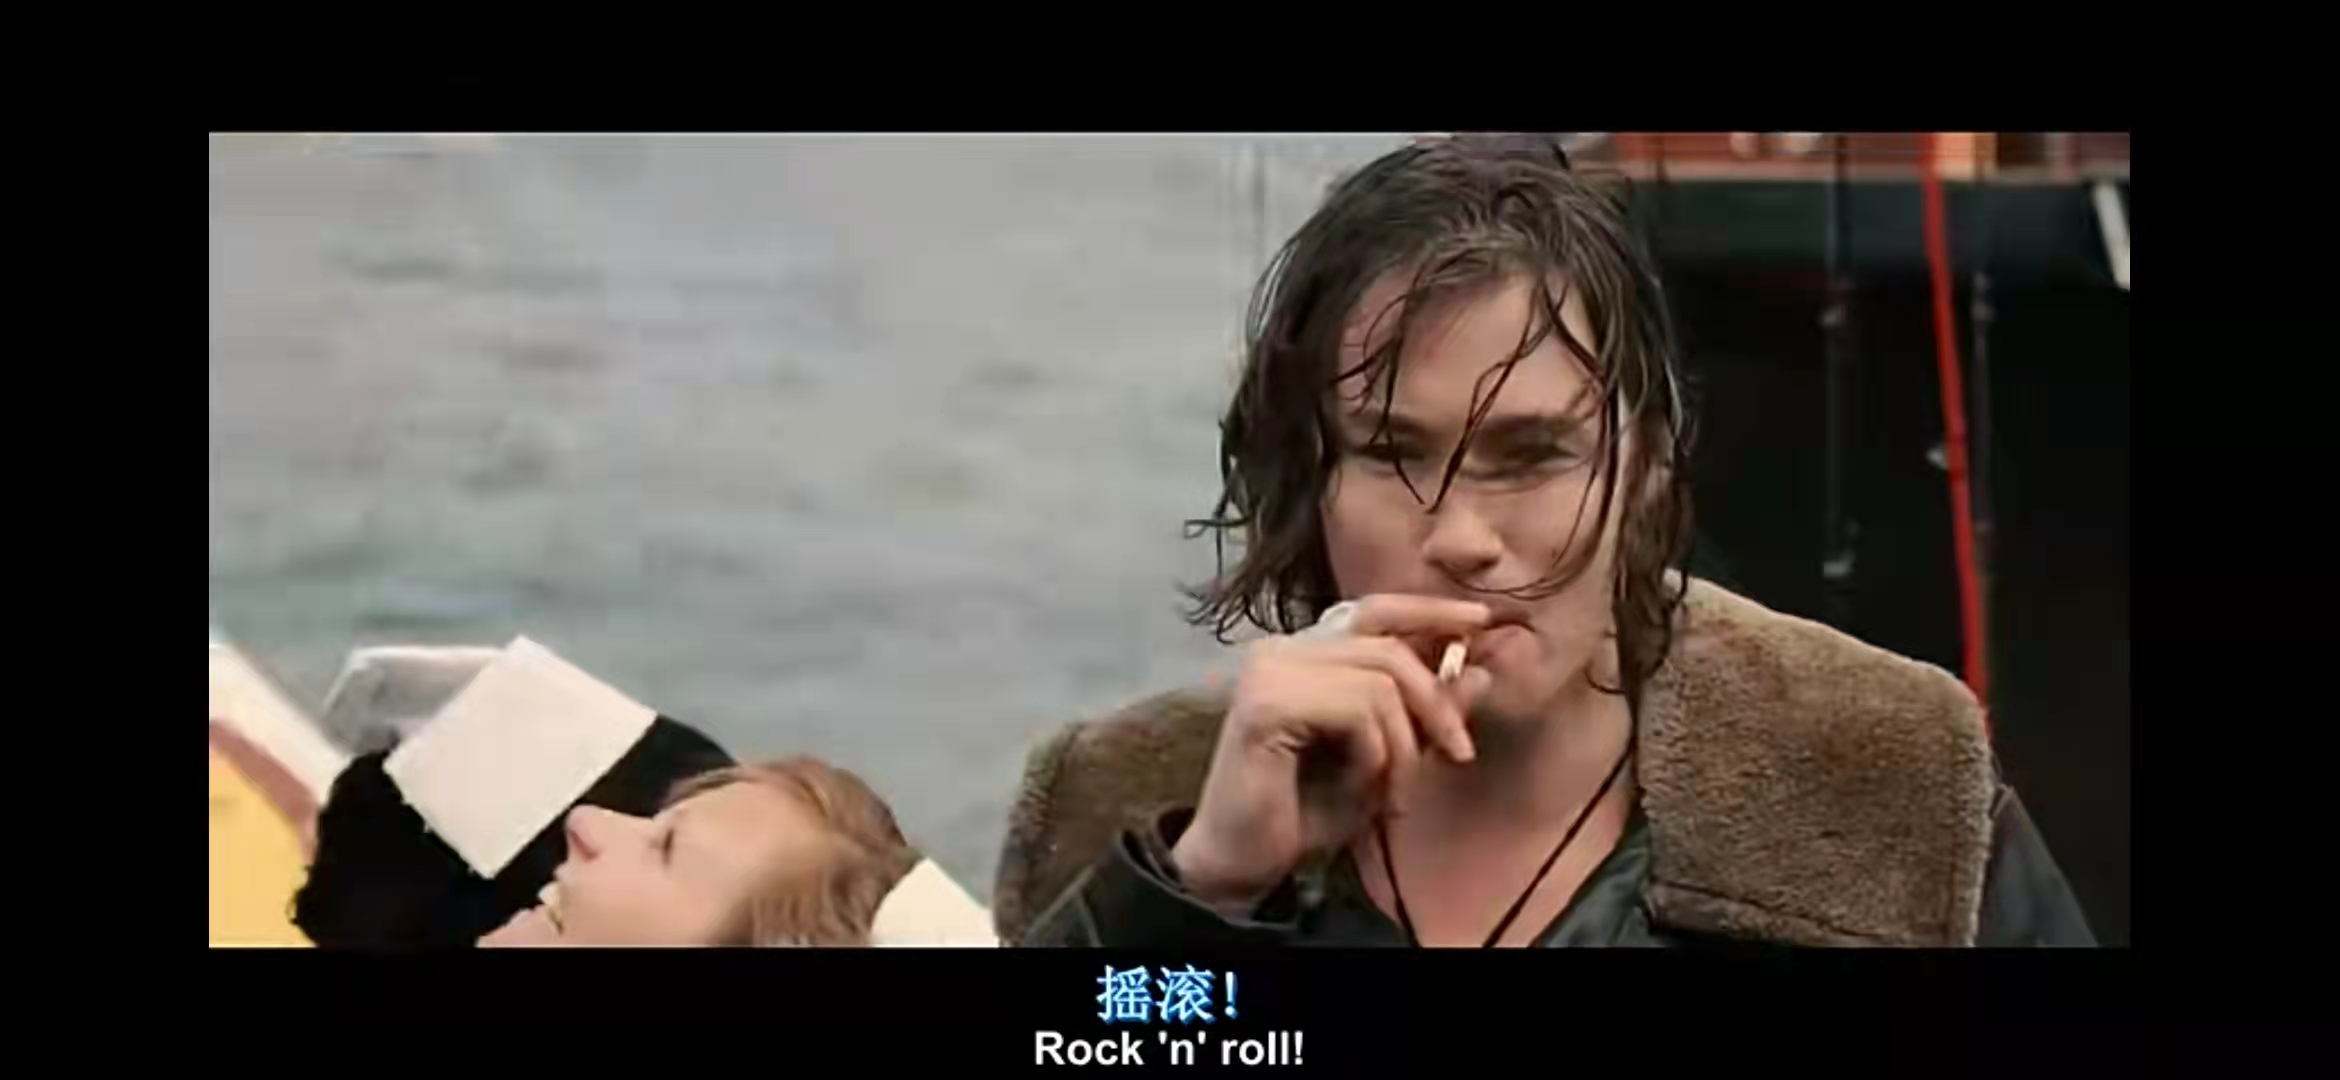
\includegraphics[scale=0.05]{fig/5}\label{4}
		}
		\caption{热力学量随时间变化曲线图} %四个子图组成的图片的批注
	\end{figure}
	
\end{document}
